\chapter{クイズの解答例}

% ==============================================================
\subsection*{第2章 データベースの基礎知識}
% ==============================================================

\subsubsection*{Q1. メジャーなデータベース管理システム}
代表的なDBMSを以下に挙げる．

\begin{itemize}
    \item \textbf{関係データベース管理システム（RDBMS）}:
    \begin{itemize}
        \item \textbf{MySQL}：世界で最も普及しているオープンソースのRDBMSの一つ．ウェブアプリケーションのバックエンドとして広く利用される．
        \item \textbf{PostgreSQL}：高機能なオープンソースのRDBMS．標準SQLへの準拠度が高く，地理情報処理など拡張機能も豊富．
        \item \textbf{Oracle Database}：大企業向けの商用RDBMSの代表格．高可用性・高性能が特長．
        \item \textbf{Microsoft SQL Server}：Microsoftが開発する商用RDBMS．Windowsおよびエンタープライズ環境での利用が多い．
        \item \textbf{SQLite}：サーバプロセスを必要としない軽量なRDBMS．スマートフォンアプリや組込みシステムで広く利用される．
    \end{itemize}
    \item \textbf{非関係型データベース管理システム（NoSQL DBMS）}:
    \begin{itemize}
        \item \textbf{MongoDB}（ドキュメント型）：JSONに近い形式でデータを管理する．スキーマが柔軟で，多様な構造のデータを扱いやすい．
        \item \textbf{Redis}（キーバリュー型）：キーと値のペアでデータを管理するインメモリDBMS．非常に高速で，セッション管理やキャッシュ処理に利用される．
        \item \textbf{Apache Cassandra}（ワイドカラム型）：大規模分散システム向けのDBMS．高可用性とスケーラビリティが特長．
        \item \textbf{Neo4j}（グラフ型）：ノードとエッジからなるグラフ構造でデータを管理する．ソーシャルネットワーク分析や知識グラフの構築に利用される．
    \end{itemize}
\end{itemize}

\subsubsection*{Q2. 線形探索}
目的の商品がリストのいずれかの位置に等確率（一様分布）で存在すると仮定する．
商品がリストの $k$ 番目（$k = 1, 2, \ldots, n$）に存在するとき，線形探索では $k$ 回の確認が必要となる．

全体の平均確認回数は
\begin{equation}
\frac{1}{n} \sum_{k=1}^{n} k = \frac{1}{n} \cdot \frac{n(n+1)}{2} = \frac{n+1}{2}
\end{equation}
となる．$n = 1{,}000{,}000$ のとき，
\begin{equation}
\frac{1{,}000{,}000 + 1}{2} = 500{,}000.5 \approx 500{,}001 \text{ 回}
\end{equation}
すなわち，\textbf{平均して約50万回}の確認が必要となる．

なお，目的の商品がリストに存在しない場合は，末尾まで確認しても見つからないため，常に $n = 1{,}000{,}000$ 回の確認が必要となる．

\subsubsection*{Q3. データベース管理システムの利用例}
例として以下が挙げられる（それ以外にも銀行の取引管理，病院の患者情報管理，スマートフォンの連絡先管理など多数考えられる）：
\begin{enumerate}
    \item \textbf{オンラインショッピングサービス}（例：Amazonなど）：商品情報，在庫数量，ユーザのアカウント情報，注文・配送履歴などをデータベースで管理している．
    \item \textbf{SNSサービス}（例：X（旧Twitter）など）：ユーザのプロフィール情報，投稿内容，フォロー・フォロワーの関係などをデータベースで管理している．
    \item \textbf{交通系ICカードのサービス}（例：SuicaやTOICAなど）：利用者のカード情報，乗降履歴，残高情報などをデータベースで管理している．
\end{enumerate}

\subsubsection*{Q4. CSV/TSVファイル}
\textbf{CSVファイル}（Comma-Separated Values）は，各行のデータ項目をカンマ（,）で区切ったテキストファイルである．\textbf{TSVファイル}（Tab-Separated Values）は，区切り文字にタブ文字を使う点がCSVと異なる．どちらも表形式のデータを保存・共有するために広く使われている形式である．

CSV/TSVファイルをDBMSの代わりにデータ管理に用いた場合の主な欠点：
\begin{enumerate}
    \item \textbf{大規模データの高速処理が困難}：特定のレコードを探すには原則としてファイルを先頭から全件読み込む必要があり，データ量が増えると処理が著しく遅くなる（索引付けができない）．
    \item \textbf{データ型・制約の定義・自動検証ができない}：数値として扱うべき列に文字列が混入したり，必須項目（NOT NULL）が空欄になっても，自動チェック機構がないため，不正なデータが混入しやすい．
    \item \textbf{同時アクセスの制御ができない}：複数のユーザが同時にファイルへの書き込みを行うと，データが上書きされて破損する可能性がある（排他制御の仕組みがない）．
    \item \textbf{テーブル間の参照整合性を保証できない}：複数のCSVファイルにまたがるデータの整合性（例：注文ファイルに存在する商品IDが商品ファイルにも必ず存在するという保証）を自動では管理できない．
\end{enumerate}

\subsubsection*{Q5. チューリング賞}
データベースに関する功績でチューリング賞を受賞した，Edgar F. Codd氏以外の代表的な受賞者を以下に挙げる：
\begin{itemize}
    \item \textbf{Charles W. Bachman（1973年受賞）}：世界初のDBMSとされるIDS（Integrated Data Store）を設計・開発し，ネットワーク型データベースを確立した功績が評価された．
    \item \textbf{Jim Gray（1998年受賞）}：データベースのトランザクション処理に関する先駆的な研究（ACIDプロパティの定式化，障害回復手法など）への貢献が評価された．
    \item \textbf{Michael Stonebraker（2014年受賞）}：オープンソースRDBMSのIngresおよびPostgresの開発を通じ，オブジェクト関係モデルや拡張可能なDBMSなど，現代的なデータベース技術の概念実証と普及に大きく貢献した功績が評価された．
\end{itemize}


% ==============================================================
\subsection*{第3章 関係データモデル}
% ==============================================================

\subsubsection*{Q1. 直積}
$|S_{lang}| = 3$，$|S_{popularity}| = 2$，$|S_{difficulty}| = 3$ より，$S_{lang} \times S_{popularity} \times S_{difficulty}$ の要素数は $3 \times 2 \times 3 = 18$ である．全要素を列挙すると以下の18タプルとなる：
\begin{align*}
&(Python,\; 人気,\; 難),\quad (Python,\; 人気,\; 普通),\quad (Python,\; 人気,\; 易), \\
&(Python,\; 不人気,\; 難),\quad (Python,\; 不人気,\; 普通),\quad (Python,\; 不人気,\; 易), \\
&(R,\; 人気,\; 難),\quad (R,\; 人気,\; 普通),\quad (R,\; 人気,\; 易), \\
&(R,\; 不人気,\; 難),\quad (R,\; 不人気,\; 普通),\quad (R,\; 不人気,\; 易), \\
&(C++,\; 人気,\; 難),\quad (C++,\; 人気,\; 普通),\quad (C++,\; 人気,\; 易), \\
&(C++,\; 不人気,\; 難),\quad (C++,\; 不人気,\; 普通),\quad (C++,\; 不人気,\; 易)
\end{align*}

\subsubsection*{Q2. 関係}
Q1の直積集合の任意の部分集合が3項関係となる（正解は多数あり，一意に決まらない）．
一例として，「各プログラミング言語に関するある学習者の主観的評価」を表す関係 $R$ を以下のように定義する：
\begin{equation*}
R = \{(Python,\; 人気,\; 易),\quad (R,\; 人気,\; 普通),\quad (C^{++},\; 不人気,\; 難)\}
\end{equation*}
これは $S_{lang} \times S_{popularity} \times S_{difficulty}$ の部分集合（$R \subseteq S_{lang} \times S_{popularity} \times S_{difficulty}$）となっており，3項関係の定義を満たす．

\subsubsection*{Q3. 関係スキーマ}
関係スキーマ $\textbf{学生}(\underline{学籍番号},\; 氏名,\; 学部,\; 年齢,\; 出身都道府県)$ に従う表データの例（見出し行を含む）を以下に示す．

\begin{table}[!htbp]
    \centering
    \begin{tabular}{lllrl}
    \toprule
    \textbf{学籍番号} & \textbf{氏名} & \textbf{学部} & \textbf{年齢} & \textbf{出身都道府県} \\ \midrule
    B21001 & 山田 太郎 & 工学部   & 20 & 愛知県 \\
    B21002 & 田中 花子 & 文学部   & 19 & 東京都 \\
    B22001 & 鈴木 一郎 & 理学部   & 21 & 大阪府 \\
    B22002 & 佐藤 美咲 & 経済学部 & 22 & 福岡県 \\
    B23001 & 伊藤 健   & 情報学部 & 18 & 北海道 \\ \bottomrule
    \end{tabular}
\end{table}

\subsubsection*{Q4. ドメイン}
Q3の関係スキーマ「学生」の各属性のドメインを定義する例を以下に示す（ドメインの定義は設計者の判断によって変わりうる）：
\begin{align*}
Dom(\text{学籍番号}) &= \{ s \mid s \in \text{'B' + 5桁の数字からなる文字列} \} \\
Dom(\text{氏名}) &= \{ s \mid s \in \text{日本語の姓名を表す文字列}\} \\
Dom(\text{学部}) &= \{\text{工学部}, \text{文学部}, \text{理学部}, \text{経済学部}, \text{法学部}, \text{医学部}, \text{情報学部} \} \\
Dom(\text{年齢}) &= \{ x \in \mathbb{N} \mid 18 \leq x \leq 30 \} \\
Dom(\text{出身都道府県}) &= \{\text{北海道}, \text{青森県}, \text{岩手県}, \ldots, \text{沖縄県}\} \quad \text{（日本の47都道府県）}
\end{align*}

\subsubsection*{Q5. ドメイン制約}
Q4で定義したドメインに違反するタプルの例を以下に挙げる：
\begin{enumerate}
    \item $('B21001',\; \text{'山田 太郎'},\; \text{'工学部'},\; -1,\; \text{'愛知県'})$：属性「年齢」の値 $-1$ が $Dom(\text{年齢})$ に含まれていない（年齢が負）のでドメイン制約違反．
    \item $('21001',\; \text{'田中 花子'},\; \text{'文学部'},\; 20,\; \text{'東京都'})$：属性「学籍番号」の値が 'B' で始まっておらず $Dom(\text{学籍番号})$ に含まれていないためドメイン制約違反．
    \item $('B22001',\; \text{'鈴木 一郎'},\; \text{'スポーツ学部'},\; 21,\; \text{'名古屋'})$：「スポーツ学部」は $Dom(\text{学部})$ に含まれておらず，「名古屋」は市名であり $Dom(\text{出身都道府県})$ にも含まれていないため，2つのドメイン制約違反が生じている．
\end{enumerate}

\subsubsection*{Q6. 超キーと候補キー}
関係スキーマ $\boldsymbol{R}(A, B, C, D)$ において主キーが $\{A, B\}$ であるということは，$\{A, B\}$ が候補キーであることを意味する．各選択肢を検討する：
\begin{enumerate}
    \item $\{A\}$：主キー $\{A, B\}$ の真部分集合であり，$A$ の値だけでは全タプルを一意に識別できない．よって\textbf{超キーではない}．
    \item $\{A, B\}$：主キーそのものであり，超キーかつ候補キーである．「超キーではあるが候補キーでない」には\textbf{該当しない}．
    \item $\{A, C\}$：$A$ と $C$ の組み合わせでタプルを一意に識別できるかどうかは問題文の情報からは判断できないため，\textbf{解答対象外}．
    \item $\{A, B, C\}$：候補キー $\{A, B\}$ を真部分集合として含む上位集合であるため超キーである．しかし $C$ を除いても超キーのままであり，最小性を満たさないため候補キーではない．よって\textbf{超キーではあるが候補キーでない}（正解）．
    \item $\{A, B, C, D\}$：候補キー $\{A, B\}$ を真部分集合として含む上位集合であるため超キーである．$C$ や $D$ を除いても超キーのままであり，最小性を満たさないため候補キーではない．よって\textbf{超キーではあるが候補キーでない}（正解）．
\end{enumerate}
\textbf{正解：4と5}（$\{A, B, C\}$ と $\{A, B, C, D\}$）．

\subsubsection*{Q7. 候補キー2}
\begin{enumerate}
    \item 制約条件から導かれる関数従属性を以下にすべて列挙する：
        \begin{itemize}
            \item 「各従業員は重複のない従業員番号を1つだけもつ」より，従業員番号の値が決まれば各従業員の情報（従業員名，部門コード，生年月日，住所）が一意に決まる．
            \item 「1人の従業員が所属する部門は1つだけ」より，従業員番号 $\to$ 部門コードが成り立つ．
            \item 「同姓同名の従業員がいてもよい」より，従業員名 $\not\to$ 従業員番号 が成り立つ（従業員名は一意識別子にならない）．
            \item 「1つの部門には複数名の従業員が所属する」より，部門コード $\not\to$ 従業員番号 が成り立つ（部門コードだけでは従業員を特定できない）．
        \end{itemize}
        以上をまとめると，成立する関数従属性は以下の1つである：
        \begin{equation}
        \text{従業員番号} \to \{\text{従業員名},\; \text{部門コード},\; \text{生年月日},\; \text{住所}\}
        \end{equation}
    \item 上記の関数従属性から，属性「従業員番号」の値が決まれば残りのすべての属性の値が一意に決まる．また，従業員番号だけで全属性を決定できるため最小性も満たす．よって，関係「従業員」の候補キーは $\{\text{従業員番号}\}$ のみである．
\end{enumerate}

\subsubsection*{Q8. 主キー}
各属性の組み合わせを検討する．

$\{\text{店舗コード}, \text{会員番号}\}$ を候補として検討すると，表中には (店舗コード$=$'S02', 会員番号$=$1) という値の組が「八事」と「御器所」の2行に存在する．よって $\{\text{店舗コード}, \text{会員番号}\}$ は各行を一意に識別できず，主キーにはなれない．

一方，$\{\text{店舗名}, \text{会員番号}\}$ を検討すると，表中のすべての（店舗名，会員番号）の組は一意であり，かつ店舗名のみでも会員番号のみでも一意識別はできない（最小性を満たす）．

よって，想定される主キーは $\boldsymbol{\{\text{店舗名}, \text{会員番号}\}}$ である．

\subsubsection*{Q9. 参照整合性制約}
5つのテーブルからなるデータベースにおいて定義すべき参照整合性制約は以下の4つである：
\begin{align}
&\pi_{\text{商品カテゴリID}}(\textbf{商品}) \subseteq \pi_{\text{商品カテゴリID}}(\textbf{商品カテゴリ}) \\
&\pi_{\text{顧客ID}}(\textbf{購買}) \subseteq \pi_{\text{顧客ID}}(\textbf{顧客}) \\
&\pi_{\text{店舗ID}}(\textbf{購買}) \subseteq \pi_{\text{店舗ID}}(\textbf{店舗}) \\
&\pi_{\text{商品ID}}(\textbf{購買}) \subseteq \pi_{\text{商品ID}}(\textbf{商品})
\end{align}
(1) はテーブル「商品」の属性「商品カテゴリID」に格納される値が，テーブル「商品カテゴリ」の主キーとして必ず存在することを表す制約である．(2)〜(4) はテーブル「購買」の各外部キー属性（顧客ID，店舗ID，商品ID）の値が，それぞれの参照先テーブルの主キーとして必ず存在することを表す制約である．


% ==============================================================
\subsection*{第4章 SQL - その1}
% ==============================================================

以下のSQL文はいずれも \graybox{SSDSE.db} 内のテーブル \graybox{population} を対象とする．テーブル \graybox{population} の列名は \graybox{地域コード}，\graybox{都道府県}，\graybox{調査年度}，\graybox{総人口}，\graybox{小学校児童数}，\graybox{中学校生徒数}，\graybox{高等学校生徒数}，\graybox{大学学生数} である．

\subsubsection*{Q1. 射影}
\begin{minted}[gobble=0,
    bgcolor=background,
    fontsize=\small,
    linenos=false,
    xleftmargin=0em]{sql}
SELECT 都道府県, 調査年度, 大学学生数
FROM population
LIMIT 30;
\end{minted}

\subsubsection*{Q2. 選択 (1/3)}
\begin{minted}[gobble=0,
    bgcolor=background,
    fontsize=\small,
    linenos=false,
    xleftmargin=0em]{sql}
SELECT *
FROM population
WHERE 都道府県 = '愛知県' AND 調査年度 = 2020;
\end{minted}

\subsubsection*{Q3. 選択 (2/3)}
「300万人」は数値 \graybox{3000000} として記述し，「県で終わる」には \graybox{LIKE} 演算子を用いる．
\begin{minted}[gobble=0,
    bgcolor=background,
    fontsize=\small,
    linenos=false,
    xleftmargin=0em]{sql}
SELECT *
FROM population
WHERE 総人口 < 3000000
  AND 都道府県 LIKE '%県'
  AND 中学校生徒数 <= 高等学校生徒数;
\end{minted}

\subsubsection*{Q4. 選択 (3/3)}
Q3の条件はそのままに，\graybox{SELECT DISTINCT} で都道府県名の重複を排除する．
\begin{minted}[gobble=0,
    bgcolor=background,
    fontsize=\small,
    linenos=false,
    xleftmargin=0em]{sql}
SELECT DISTINCT 都道府県
FROM population
WHERE 総人口 < 3000000
  AND 都道府県 LIKE '%県'
  AND 中学校生徒数 <= 高等学校生徒数;
\end{minted}

\subsubsection*{Q5. ソート (1/2)}
\begin{minted}[gobble=0,
    bgcolor=background,
    fontsize=\small,
    linenos=false,
    xleftmargin=0em]{sql}
SELECT *
FROM population
WHERE 調査年度 = 2021
ORDER BY 大学学生数 DESC;
\end{minted}

\subsubsection*{Q6. ソート (2/2)}
割合を計算する際，整数同士の除算では小数点以下が切り捨てられるため，\graybox{CAST} で実数（REAL型）に変換してから除算する．
\begin{minted}[gobble=0,
    bgcolor=background,
    fontsize=\small,
    linenos=false,
    xleftmargin=0em]{sql}
SELECT *,
       CAST(大学学生数 AS REAL) / 総人口 AS 大学学生数割合
FROM population
WHERE 調査年度 = 2021
ORDER BY 大学学生数割合 DESC;
\end{minted}

\subsubsection*{Q7. GROUP BY (1/3)}
\begin{minted}[gobble=0,
    bgcolor=background,
    fontsize=\small,
    linenos=false,
    xleftmargin=0em]{sql}
SELECT 都道府県,
       AVG(大学学生数)                    AS 大学学生数平均,
       MAX(大学学生数) - MIN(大学学生数)  AS 大学学生数最大最小差
FROM population
GROUP BY 都道府県;
\end{minted}

\subsubsection*{Q8. GROUP BY (2/3)}
\graybox{WHERE} 句で先に「総人口が300万人超」の行に絞り込んでから，\graybox{GROUP BY} で調査年度ごとに集約する．
\begin{minted}[gobble=0,
    bgcolor=background,
    fontsize=\small,
    linenos=false,
    xleftmargin=0em]{sql}
SELECT 調査年度,
       AVG(小学校児童数 + 中学校生徒数)       AS 小中合計の平均,
       AVG(高等学校生徒数 - 大学学生数)       AS 高大差の平均,
       MIN(高等学校生徒数 - 大学学生数)       AS 高大差の最小値,
       MAX(高等学校生徒数 - 大学学生数)       AS 高大差の最大値
FROM population
WHERE 総人口 > 3000000
GROUP BY 調査年度;
\end{minted}

\subsubsection*{Q9. GROUP BY (3/3)}
集約後の結果に対する絞り込みには \graybox{WHERE} ではなく \graybox{HAVING} を用いる．
\begin{minted}[gobble=0,
    bgcolor=background,
    fontsize=\small,
    linenos=false,
    xleftmargin=0em]{sql}
SELECT 都道府県,
       AVG(総人口)                         AS 総人口の平均,
       AVG(高等学校生徒数)                 AS 高等学校生徒数の平均,
       AVG(大学学生数)                     AS 大学学生数の平均,
       AVG(高等学校生徒数 - 大学学生数)    AS 高大差の平均
FROM population
GROUP BY 都道府県
HAVING AVG(高等学校生徒数 - 大学学生数) <= 10000;
\end{minted}


% ==============================================================
\subsection*{第5章 データベースの異状}
% ==============================================================

\subsubsection*{Q1. 異状の分類}
テーブル「履修登録」の主キーは \{学生ID, 科目ID\} であるため，どちらか一方だけ，または両方ともNULLになるレコードは登録できない．各トラブルの分類は以下の通り：
\begin{enumerate}
    \item \textbf{挿入時異状}．新設科目「データサイエンス入門」はまだ誰も履修登録していないため，主キーの一部である「学生ID」がNULLとなり，キー制約違反でレコードを挿入できない．本来，科目の開設と学生の履修登録は独立したできごとであるにもかかわらず，テーブルの設計上，履修者なしには科目情報を登録できないという不都合が生じている．
    \item \textbf{更新時異状}．「プログラミング基礎」の担当教員が変わった場合，この科目を履修している学生全員（100人分）のレコードについて「担当教員」の値を書き換えなければならない．これはテーブル内に同一の科目・担当教員の情報が多数のレコードに重複して格納されているためである．今回のように修正漏れが発生すると，同じ科目なのに担当教員の値が異なるレコードが混在し，データに矛盾が生じる．
    \item \textbf{削除時異状}．「離散数学」を履修していた唯一の学生のレコードを削除すると，そのレコードに含まれていた科目名「離散数学」と担当教員の情報もともに失われる．本来は単に「学生の履修取り消し」という操作のはずが，「科目および担当教員の情報そのものの消去」という意図しない副作用をもたらしてしまっている．
\end{enumerate}

\subsubsection*{Q2. 更新時異状}
テーブル「営業記録」では，主キー \{ユーザ, 商品\} のペアごとに営業担当者が割り当てられており，同一の営業担当者が複数の行に登場する．営業担当者ごとの「営業成績」の値も，その担当者が関わる全行に重複して格納されている．

ここで，ある営業担当者（例：担当者「鈴木」）の今年度の営業成績が修正された場合を考える．担当者「鈴木」が複数の（ユーザ，商品）ペアを担当していれば，テーブル「営業記録」には担当者「鈴木」が登場する行が複数存在する．よって，営業成績の修正に際しては，「鈴木」が担当しているすべての行の「営業成績」の値を書き換えなければならない．

しかし，修正の際にいずれかの行を見落とした場合，テーブル「営業記録」内で同一の担当者「鈴木」に対して異なる営業成績の値が混在することになる（例：ある行では営業成績「A」，別の行では「B」）．これが更新時異状であり，どちらの値が正しいのか判断できない矛盾した状態を引き起こす．

\subsubsection*{Q3. 削除時異状}
テーブル「営業記録2」では，各行に担当者の連絡先（連絡先）と取扱商品のメーカー（メーカー）の情報が含まれている．これらの情報は，特定の（ユーザ，商品）ペアのレコードと同じ行に混在して管理されている．

ここで，あるユーザ（例：ユーザ「田辺」）が特定の商品（例：商品「ソファ」）の購入相談をキャンセルしたため，対応するレコードをテーブルから削除する場面を考える．もし「田辺，ソファ」のレコードが，テーブル「営業記録2」における「ソファ」についての唯一の記録であった場合，そのレコードを削除すると「ソファ」のメーカー情報や，担当した営業員の連絡先情報もデータベースから失われてしまう．

本来「ユーザの問い合わせキャンセル」という操作にすぎないにもかかわらず，商品・メーカー・担当者の連絡先という別のデータが意図せず消去されるのが削除時異状である．

\subsubsection*{Q4. 挿入時異状}
テーブル「営業記録3」の主キーは \{ユーザ, 商品\} であるため，何らかのユーザが商品に関心を示して初めてレコードを挿入できる．

ここで，家具販売店「八高家具」が新しいメーカー（例：メーカー「北欧家具社」）の新商品（例：商品「ダイニングテーブル」）を取り扱い品目に追加した場面を考える．このとき，その商品に興味を持った顧客がまだ1人もいなければ，「ユーザ」の値がNULLとなりキー制約違反となるため，「北欧家具社」と「ダイニングテーブル」の対応関係をテーブル「営業記録3」に登録することができない．

本来「新商品・新メーカーの登録」という操作であるにもかかわらず，顧客（ユーザ）が現れないとメーカーと商品の情報を記録できないのが挿入時異状である．


% ==============================================================
\subsection*{第6章 関係データベースの設計 - 実体関連モデル}
% ==============================================================
\subsubsection*{Q1. 実体と関連}
図\ref{fig:ch6-q1-er-diagram}に解答例を記す．
\begin{figure}[!htbp]
    \centering
    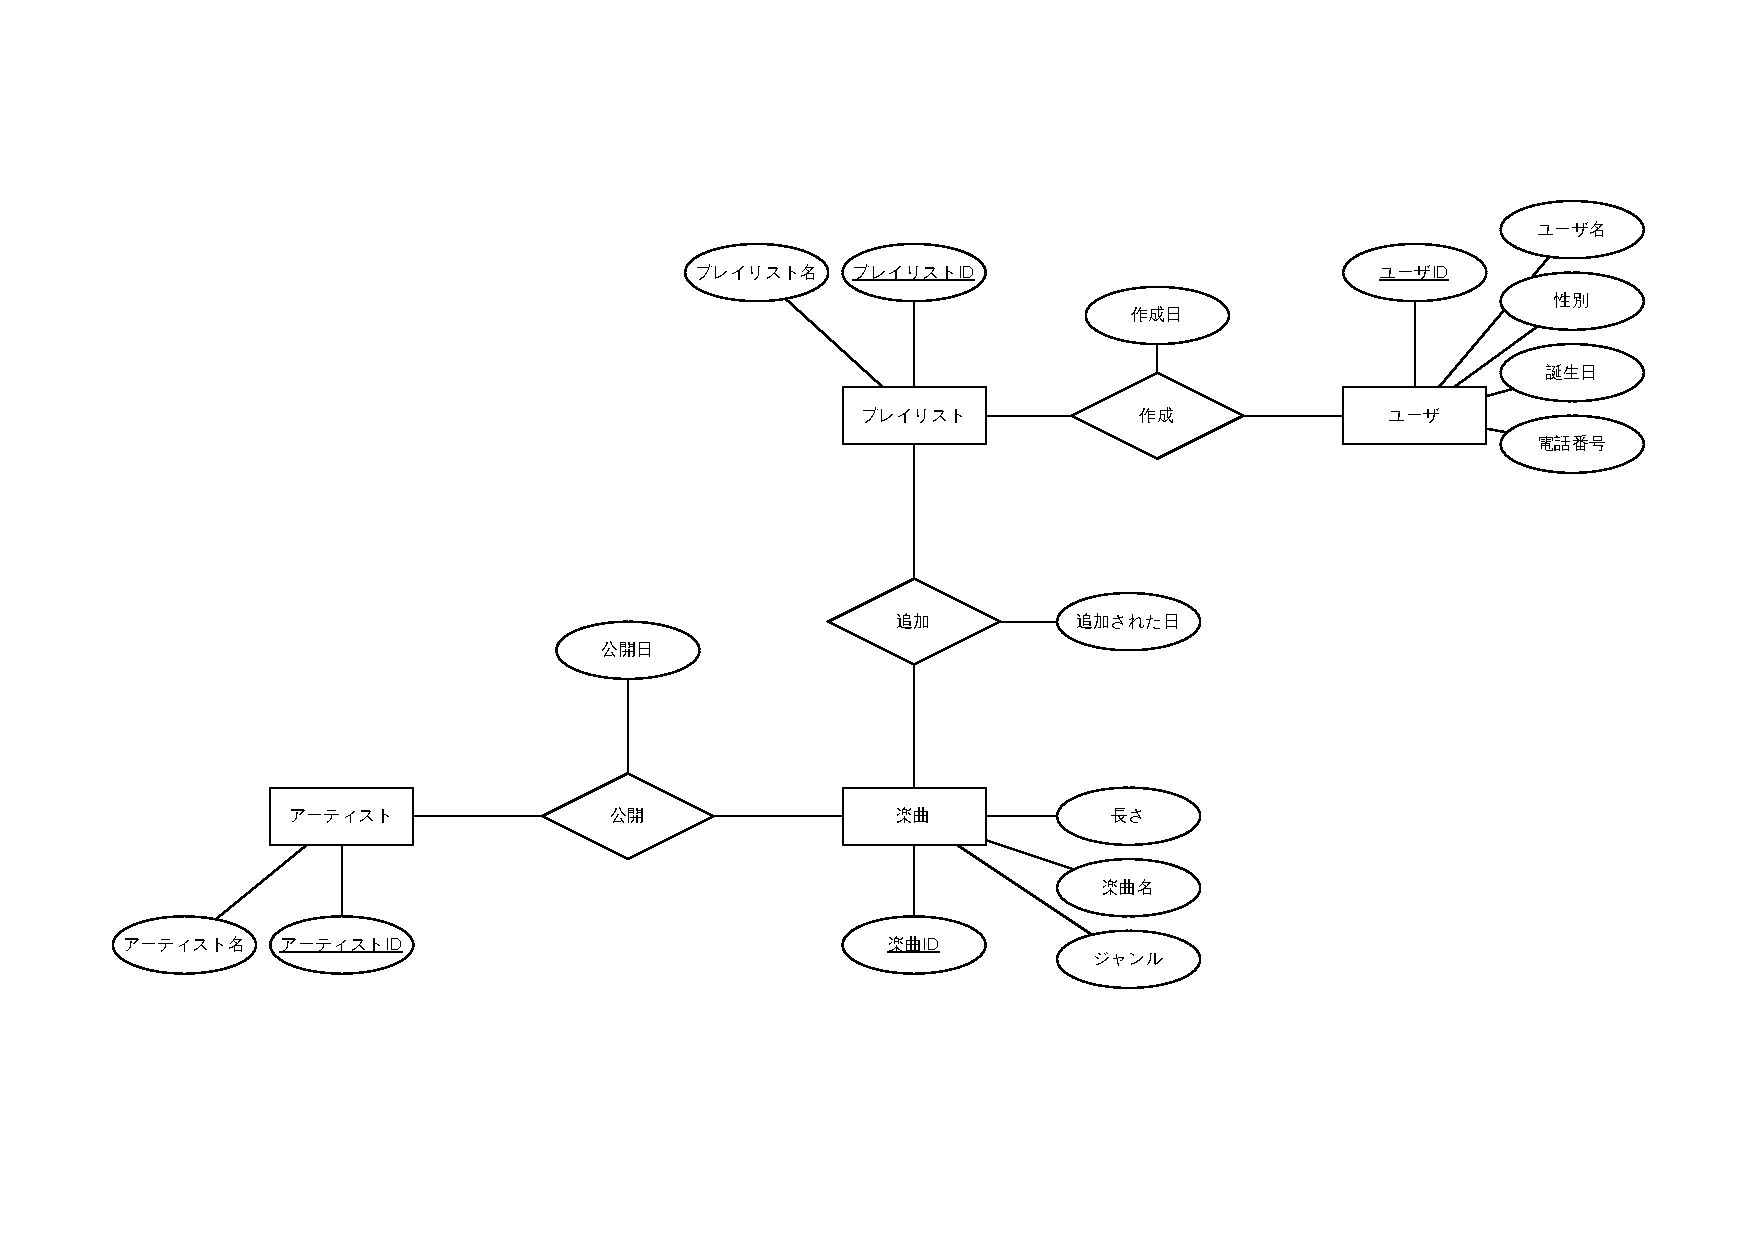
\includegraphics[width=0.90\textwidth]{figure/quiz-answer/ch6-q1.pdf}
    \caption{6章Q1のER図}
    \label{fig:ch6-q1-er-diagram}
\end{figure}

\subsubsection*{Q2. 多重度と参加制約}
図\ref{fig:ch6-q2-er-diagram}に解答例を記す．
\begin{figure}[!htbp]
    \centering
    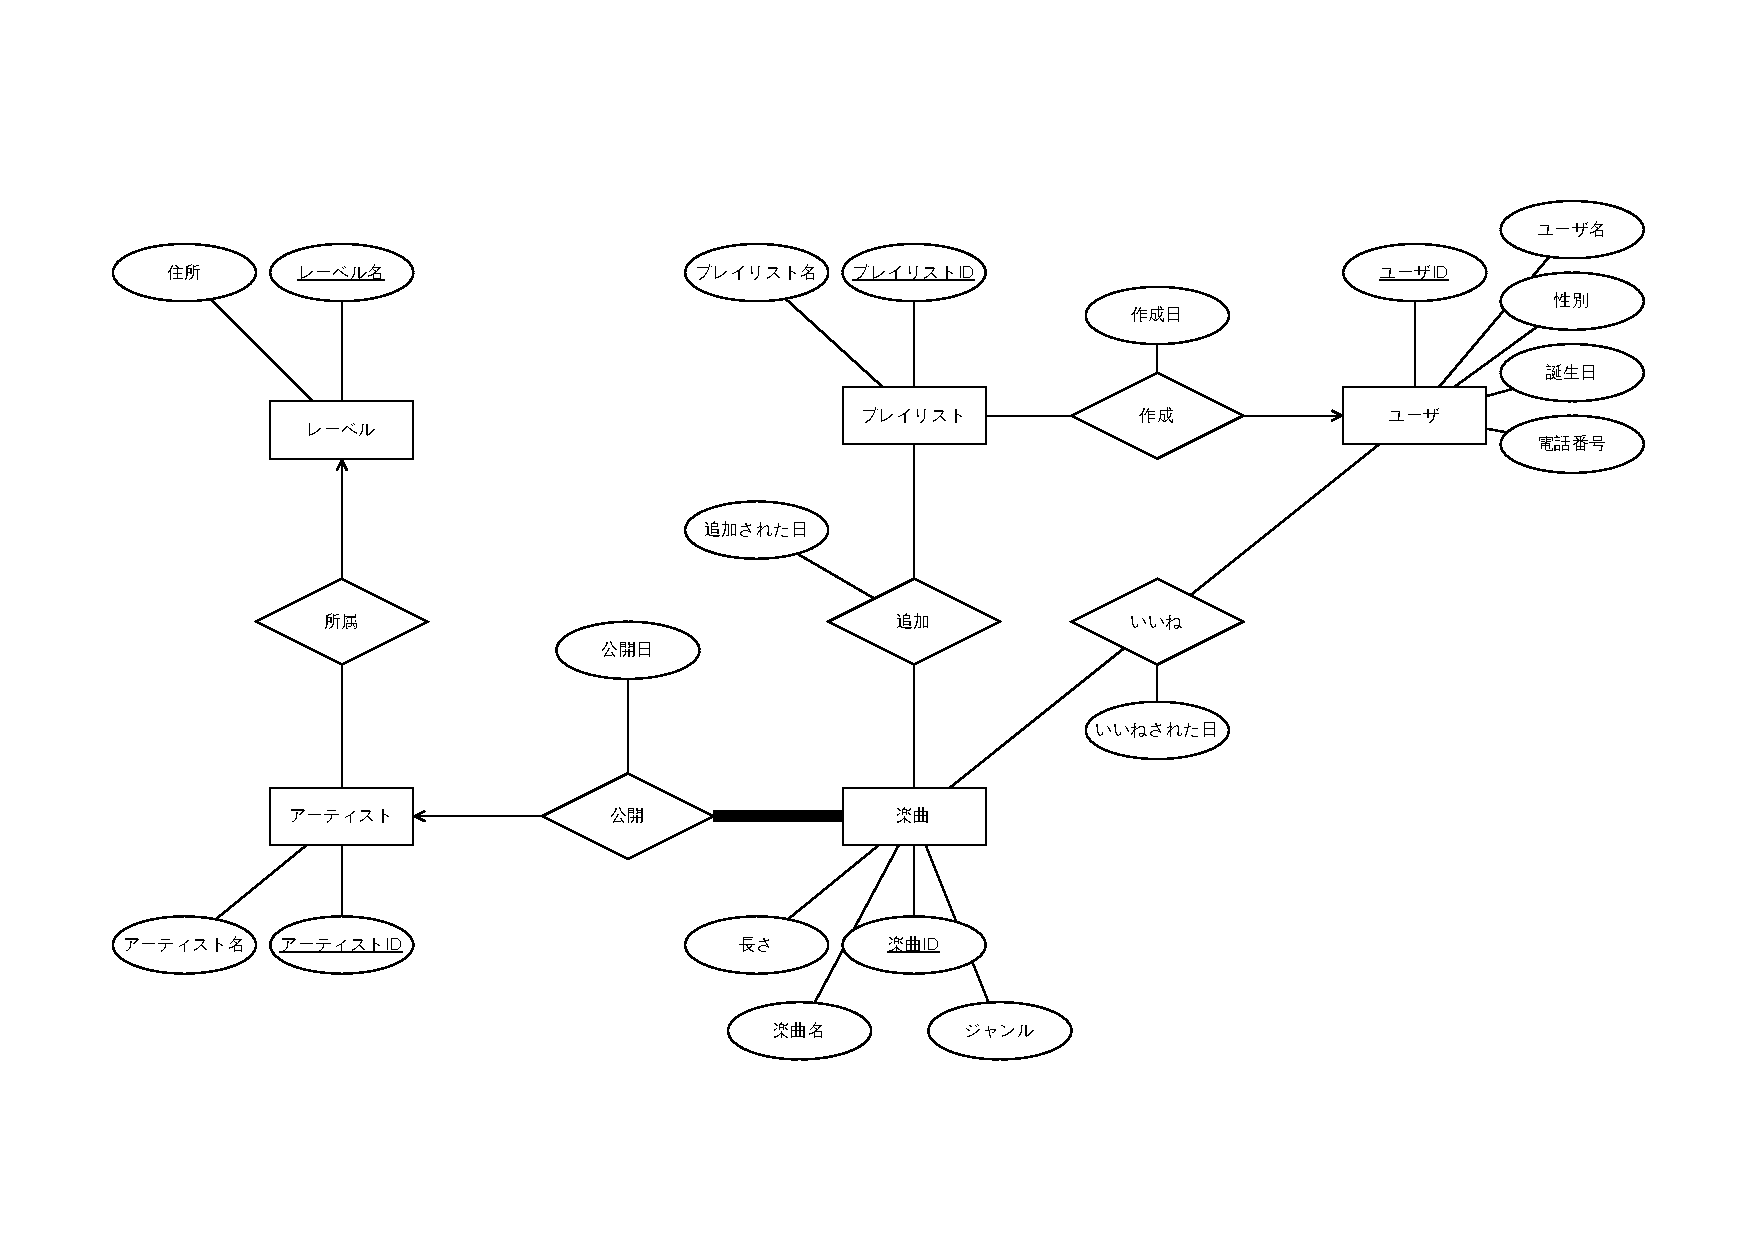
\includegraphics[width=0.90\textwidth]{figure/quiz-answer/ch6-q2.pdf}
    \caption{6章Q2のER図}
    \label{fig:ch6-q2-er-diagram}
\end{figure}

\subsubsection*{Q3. 汎化・継承}
図\ref{fig:ch6-q3-er-diagram}に解答例を記す．
\begin{figure}[!htbp]
    \centering
    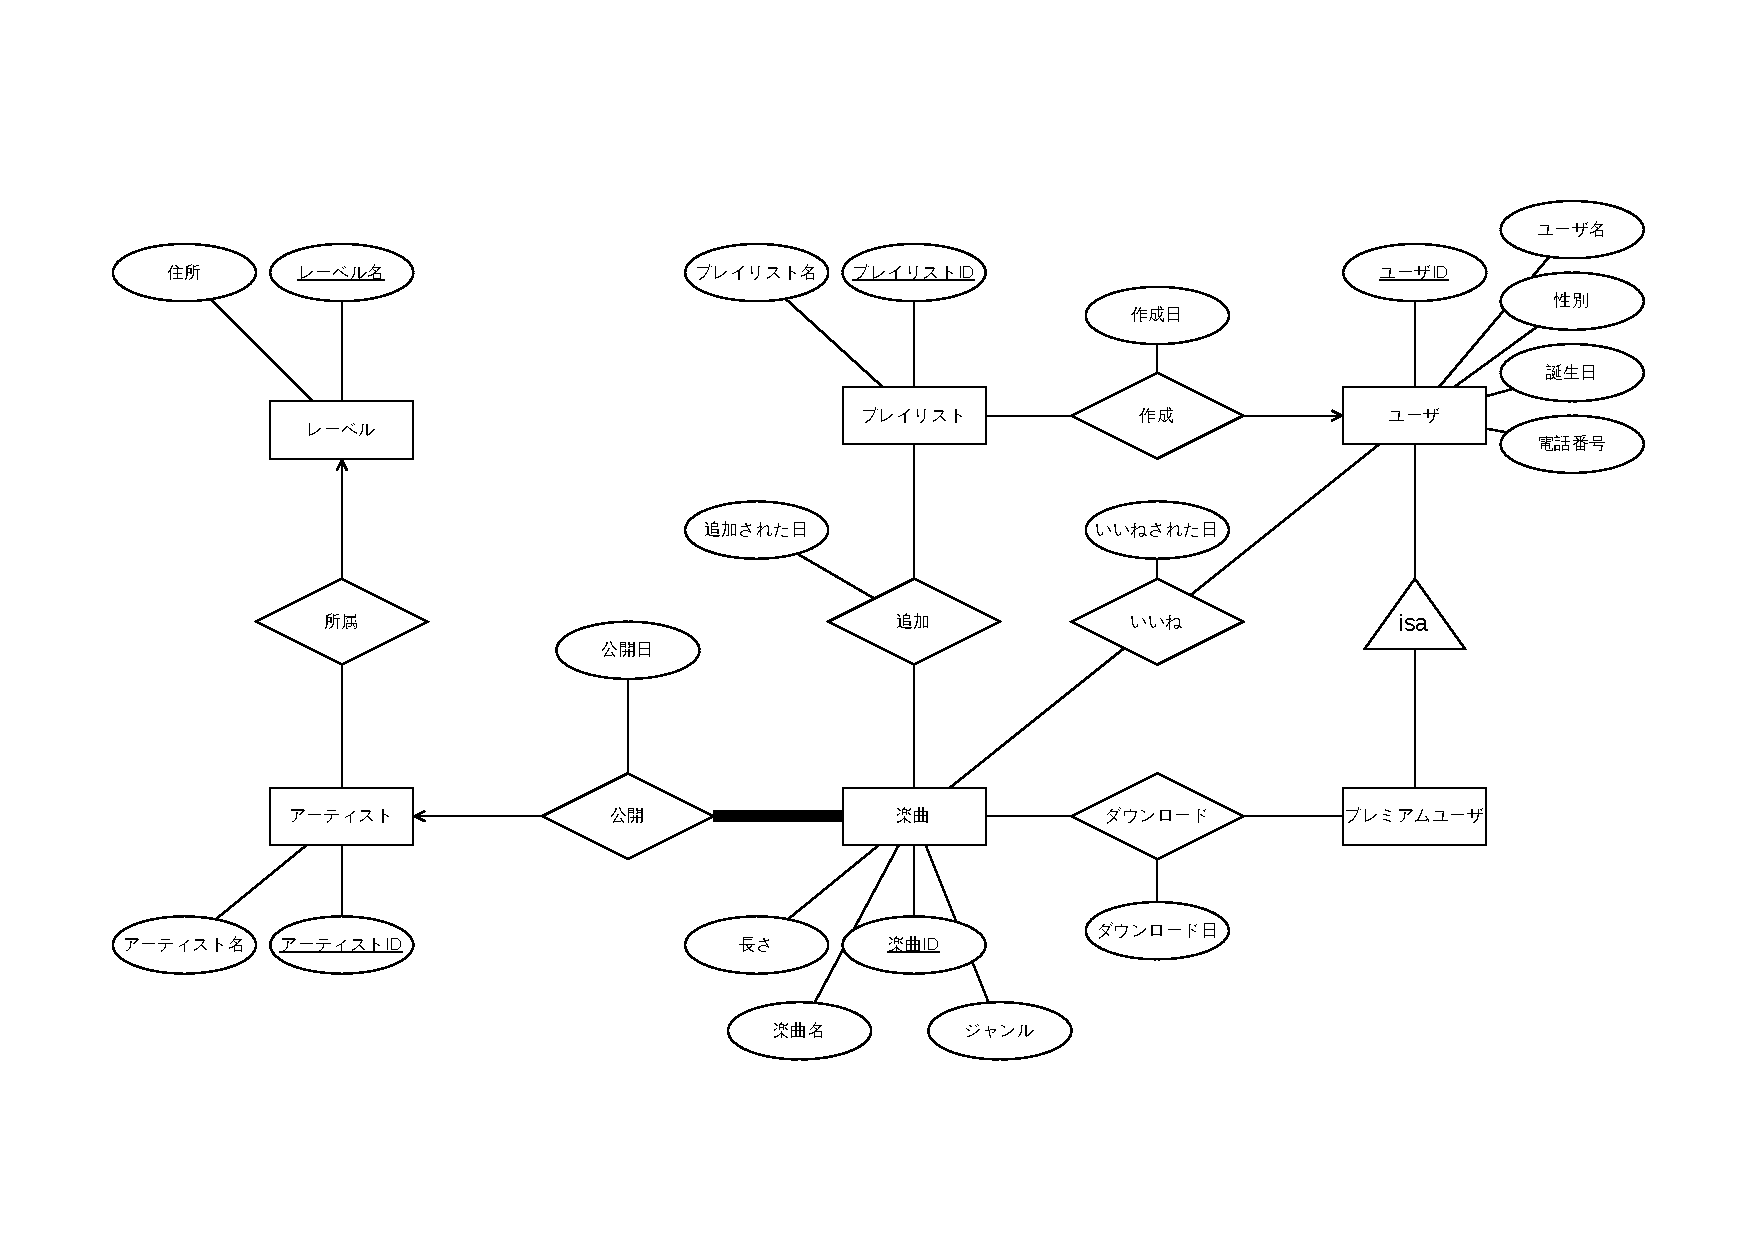
\includegraphics[width=0.90\textwidth]{figure/quiz-answer/ch6-q3.pdf}
    \caption{6章Q3のER図}
    \label{fig:ch6-q3-er-diagram}
\end{figure}

\subsubsection*{Q4. n項関連の設計}
図\ref{fig:ch6-q4-er-diagram}に解答例を記す．
\begin{figure}[!htbp]
    \centering
    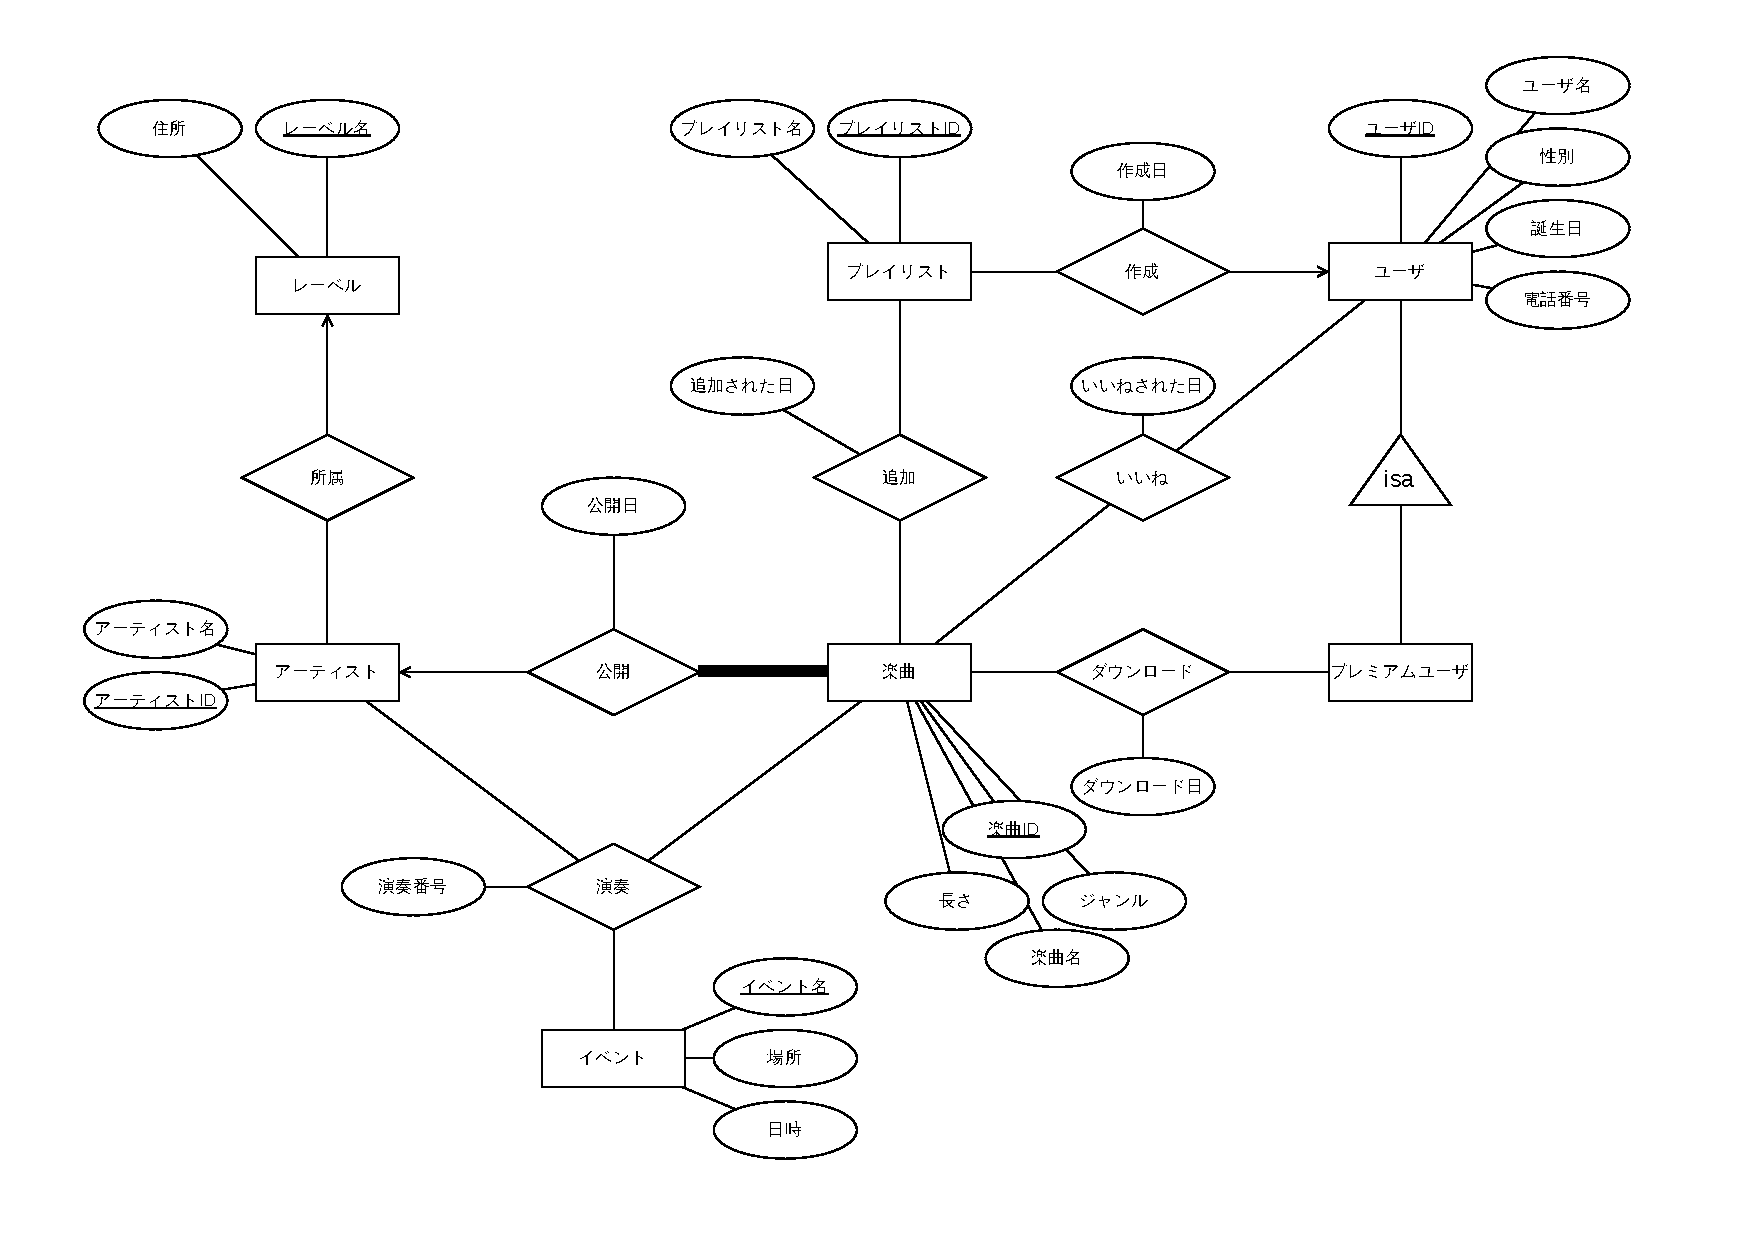
\includegraphics[width=0.90\textwidth]{figure/quiz-answer/ch6-q4.pdf}
    \caption{6章Q4のER図}
    \label{fig:ch6-q4-er-diagram}
\end{figure}

\subsubsection*{Q5. 実体関連図から関係スキーマへの変換}
図\ref{fig:erd-to-schema}のER図を変換ルールに従い，以下の6つの関係スキーマに変換する（参照整合性制約は省略）．
\begin{itemize}
    \item $\text{\textbf{ユーザ}}(\underline{\text{ユーザ名}}, \text{氏名}, \text{email}, \text{住所})$（変換パターン1）
    \item $\text{\textbf{有料会員}}(\underline{\text{ユーザ名}}, \text{登録日})$（変換パターン3；継承のためキーは継承元の「ユーザ名」）
    \item $\text{\textbf{商品}}(\underline{\text{商品ID}}, \text{商品名}, \text{発売日}, \text{価格})$（変換パターン1）
    \item $\text{\textbf{注文}}(\underline{\text{注文ID}}, \text{注文日})$（変換パターン1）
    \item $\text{\textbf{購買履歴}}(\underline{\text{注文ID}}, \text{ユーザ名})$（変換パターン2；多対1のため矢印のない「注文」側の主キーが関係のキー，「ユーザ名」は外部キー）
    \item $\text{\textbf{明細}}(\underline{\text{注文ID}, \text{商品ID}}, \text{数量})$（変換パターン2；多対多のため両実体の主キーの組がキー，「注文ID」「商品ID」はそれぞれ外部キー）
\end{itemize}

% ==============================================================
\subsection*{第7章 関係データベースの設計 - 正規化}
% ==============================================================

\subsubsection*{Q1-1: 関数従属性}
与えられた関数従属性（$FD_1$〜$FD_4$）をすべて満たす関係「評価」の例を以下に示す．

\begin{table}[!htbp]
    \centering
    \scalebox{0.70}{
    \begin{tabular}{lllll r}
    \toprule
    \textbf{ユーザ名} & \textbf{楽曲} & \textbf{アーティスト} & \textbf{収録アルバム} & \textbf{ジャンル} & \textbf{スコア} \\ \midrule
    山畑 & 白日           & King Gnu         & Sympa              & J-Pop & 5 \\
    山畑 & Bohemian Rhapsody & Queen         & A Night at the Opera & Rock  & 4 \\
    田辺 & 白日           & King Gnu         & Sympa              & J-Pop & 3 \\
    田辺 & 青と夏         & Mrs. GREEN APPLE & 青と夏（Single）   & J-Pop & 5 \\
    鈴木 & Bohemian Rhapsody & Queen         & A Night at the Opera & Rock  & 5 \\
    鈴木 & 青と夏         & Mrs. GREEN APPLE & 青と夏（Single）   & J-Pop & 4 \\ \bottomrule
    \end{tabular}
    }
\end{table}

\subsubsection*{Q1-2: FDダイアグラム}
\begin{figure}[!htbp]
    \centering
    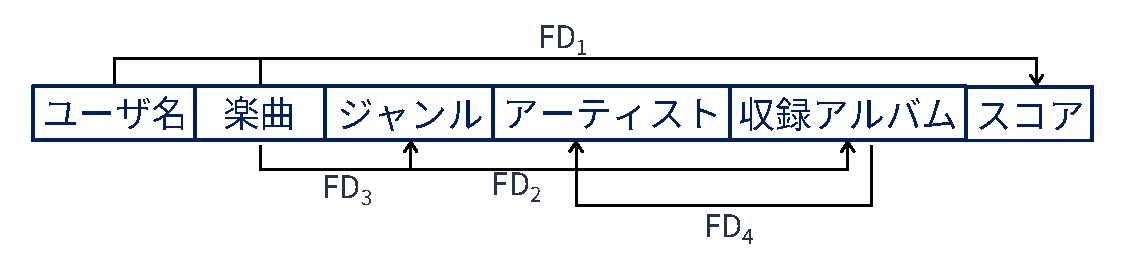
\includegraphics[width=0.90\textwidth]{figure/quiz-answer/ch7-q1-2.pdf}
    \caption{7章Q1-2のFDダイアグラム}
    \label{fig:ch7-q1-2}
\end{figure}

\subsubsection*{Q1-3: BCNFへの分解}
まず候補キーを確認する．\{ユーザ名, 楽曲\}が決まれば，$FD_1$によりスコア，$FD_2$により収録アルバム，$FD_3$によりジャンル，$FD_4$によりアーティストがすべて決定される．また，\{ユーザ名\}のみ，または\{楽曲\}のみでは全属性は決定できない．よって候補キーは$\{\text{ユーザ名, 楽曲}\}$のみである．

$FD_2$（楽曲 $\to$ 収録アルバム），$FD_3$（楽曲 $\to$ ジャンル），$FD_4$（収録アルバム $\to$ アーティスト）はいずれも左辺が候補キーでないため，BCNFに違反している．
そのため，図のように$FD_4$，$FD_2$，$FD_3$の順で分解する．

\begin{figure}[!htbp]
    \centering
    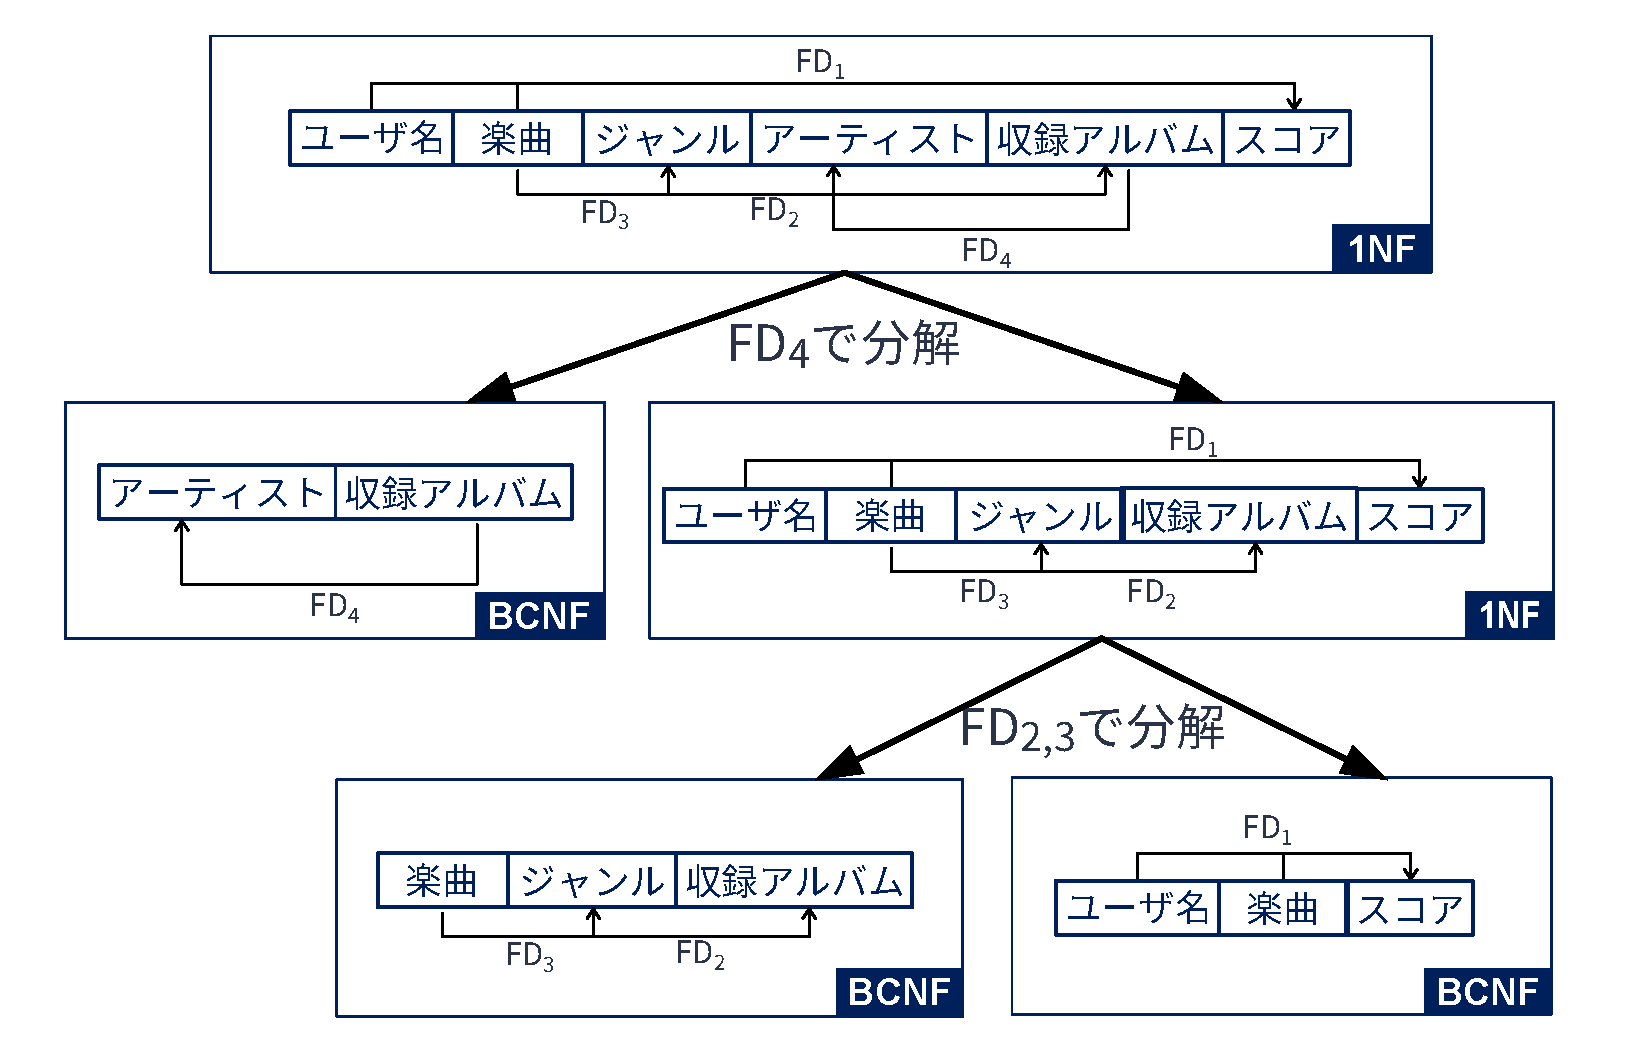
\includegraphics[width=0.90\textwidth]{figure/quiz-answer/ch7-q1-3.pdf}
    \caption{7章Q1-3の分解過程}
    \label{fig:ch7-q1-3}
\end{figure}

最終的に得られる3つのBCNFスキーマは以下の通り：
\begin{align}
    &\textbf{アルバム}(\underline{\text{収録アルバム}},\; \text{アーティスト}) \\
    &\textbf{楽曲情報}(\underline{\text{楽曲}},\; \text{収録アルバム},\; \text{ジャンル}) \\
    &\textbf{評価}(\underline{\text{ユーザ名, 楽曲}},\; \text{スコア})
\end{align}


\subsubsection*{Q2: 分解順序と結果の関係}
関係スキーマ「営業記録」：
\begin{equation*}
\textbf{営業記録}(\underline{\text{ユーザ, 商品}},\; \text{連絡先},\; \text{メーカー},\; \text{営業担当},\; \text{営業成績})
\end{equation*}
候補キー：\{ユーザ, 商品\}．$FD_2$，$FD_3$，$FD_4$の順で分解する．
分解過程は以下の図の通り．

\begin{figure}[!htbp]
    \centering
    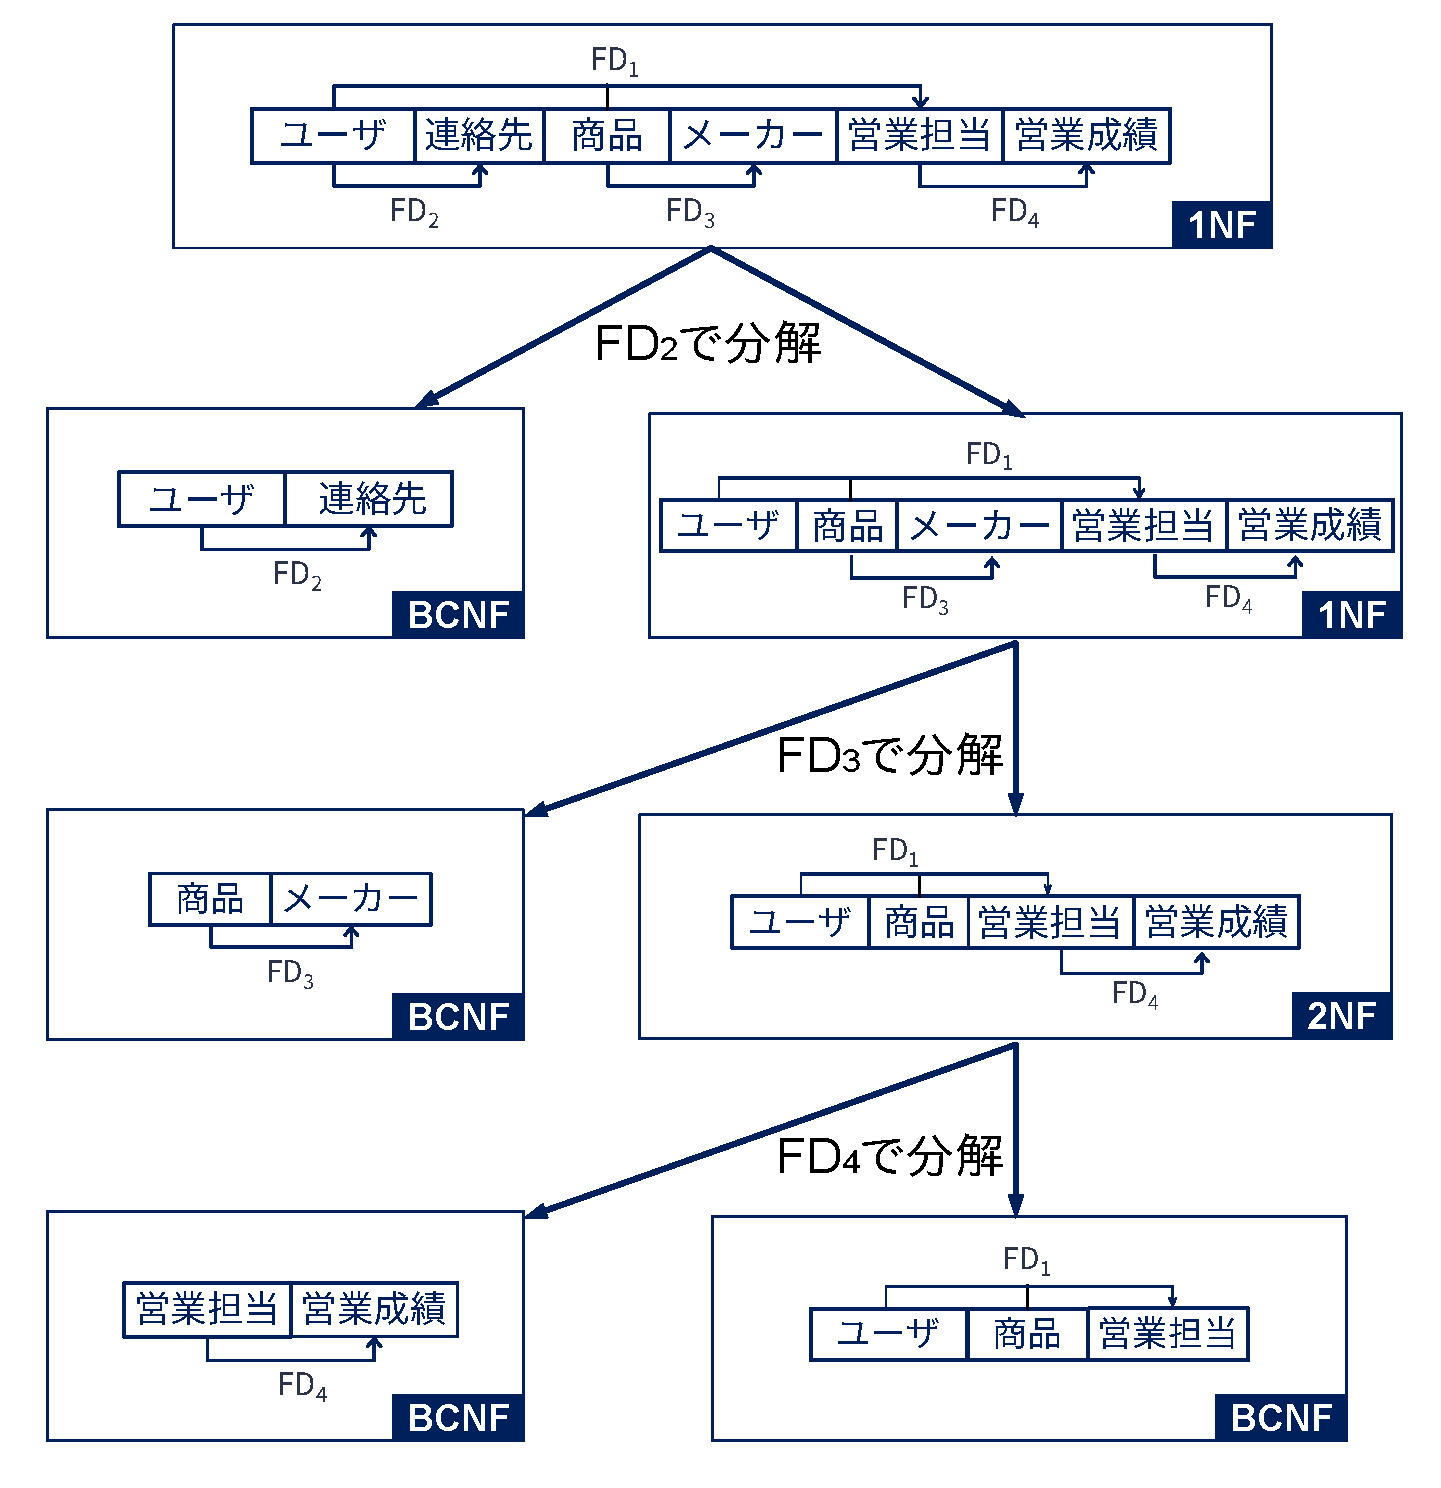
\includegraphics[width=0.90\textwidth]{figure/quiz-answer/ch7-q2.pdf}
    \caption{7章Q2の分解過程}
    \label{fig:ch7-q2}
\end{figure}

最終的に得られる4つのBCNFスキーマは，本文の例（$FD_4$，$FD_2$，$FD_3$の順）で得られた$R_6 \sim R_9$と完全に一致する：
\begin{align}
    &\boldsymbol{R_1}(\underline{\text{ユーザ, 商品}},\; \text{営業担当}) \\
    &\boldsymbol{R_2}(\underline{\text{ユーザ}},\; \text{連絡先}) \\
    &\boldsymbol{R_3}(\underline{\text{商品}},\; \text{メーカー}) \\
    &\boldsymbol{R_4}(\underline{\text{営業担当}},\; \text{営業成績})
\end{align}
このように，情報無損失分解においては関数従属性を選ぶ順序が最終結果に影響しない．


\subsubsection*{Q3: 関数従属性にもとづく正規化2}
分解過程は以下の図の通り．
\begin{figure}[!htbp]
    \centering
    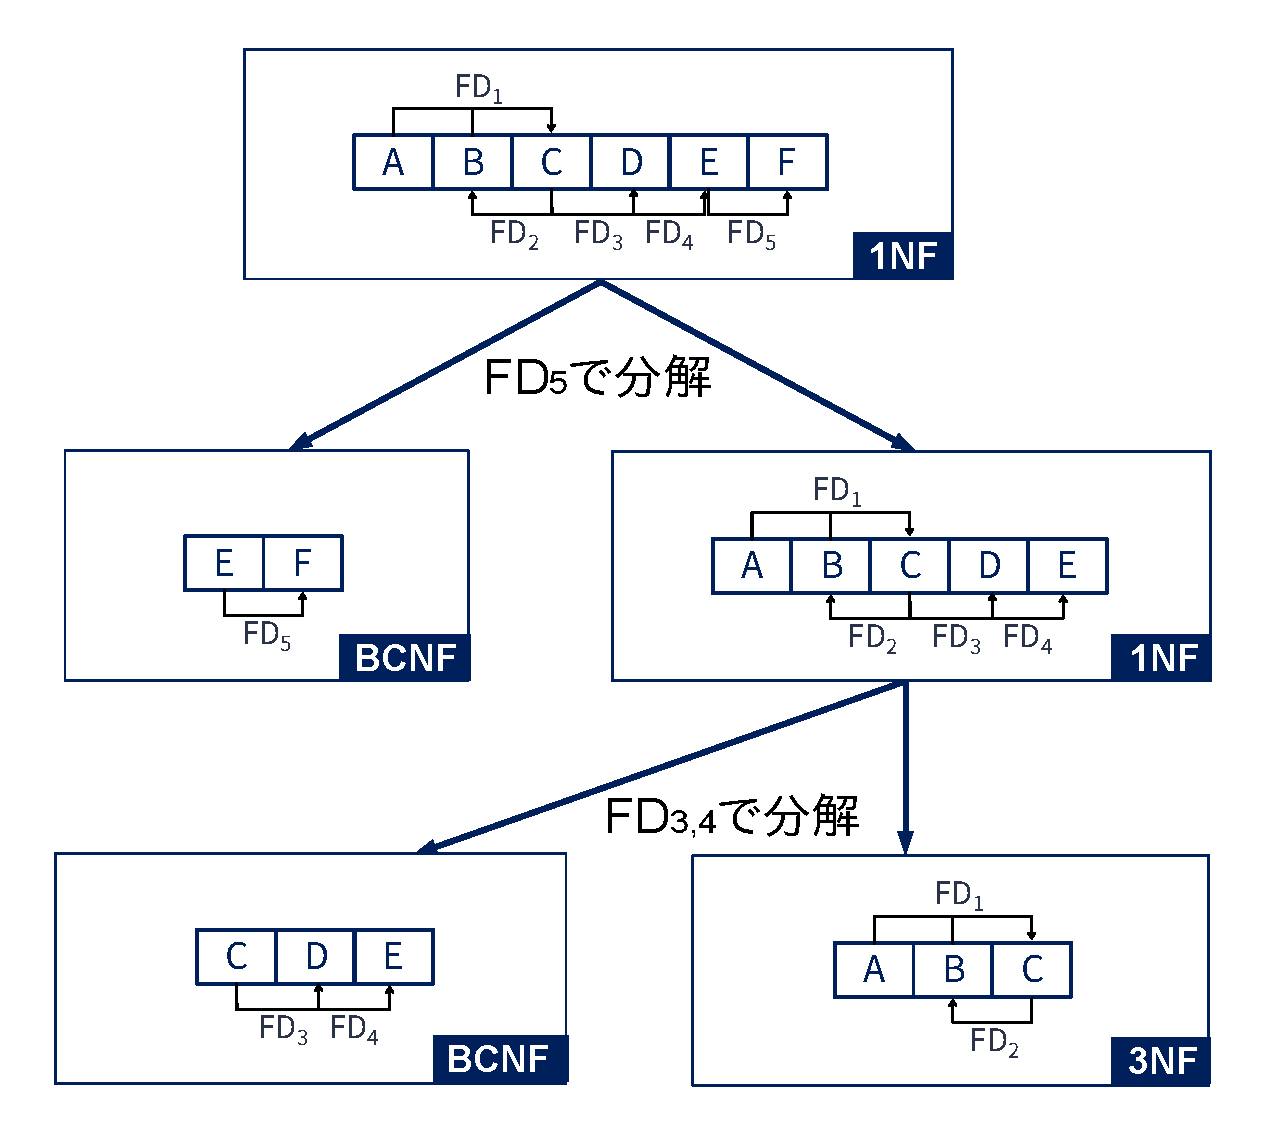
\includegraphics[width=0.90\textwidth]{figure/quiz-answer/ch7-q3.pdf}
    \caption{7章Q3の分解過程}
    \label{fig:ch7-q3}
\end{figure}

最終的に得られるスキーマ（$R_1$，$R_2$はBCNF，$R_3$は第3正規形）：
\begin{align}
    &R_1(\underline{E},\; F) \\
    &R_2(\underline{C},\; D,\; E) \\
    &R_3(A,\; B,\; C) \quad \text{（候補キー：$\{A,B\}$と$\{A,C\}$）}
\end{align}


\subsubsection*{Q4: 関数従属性にもとづく正規化3}
分解過程は以下の図の通り．
\begin{figure}[!htbp]
    \centering
    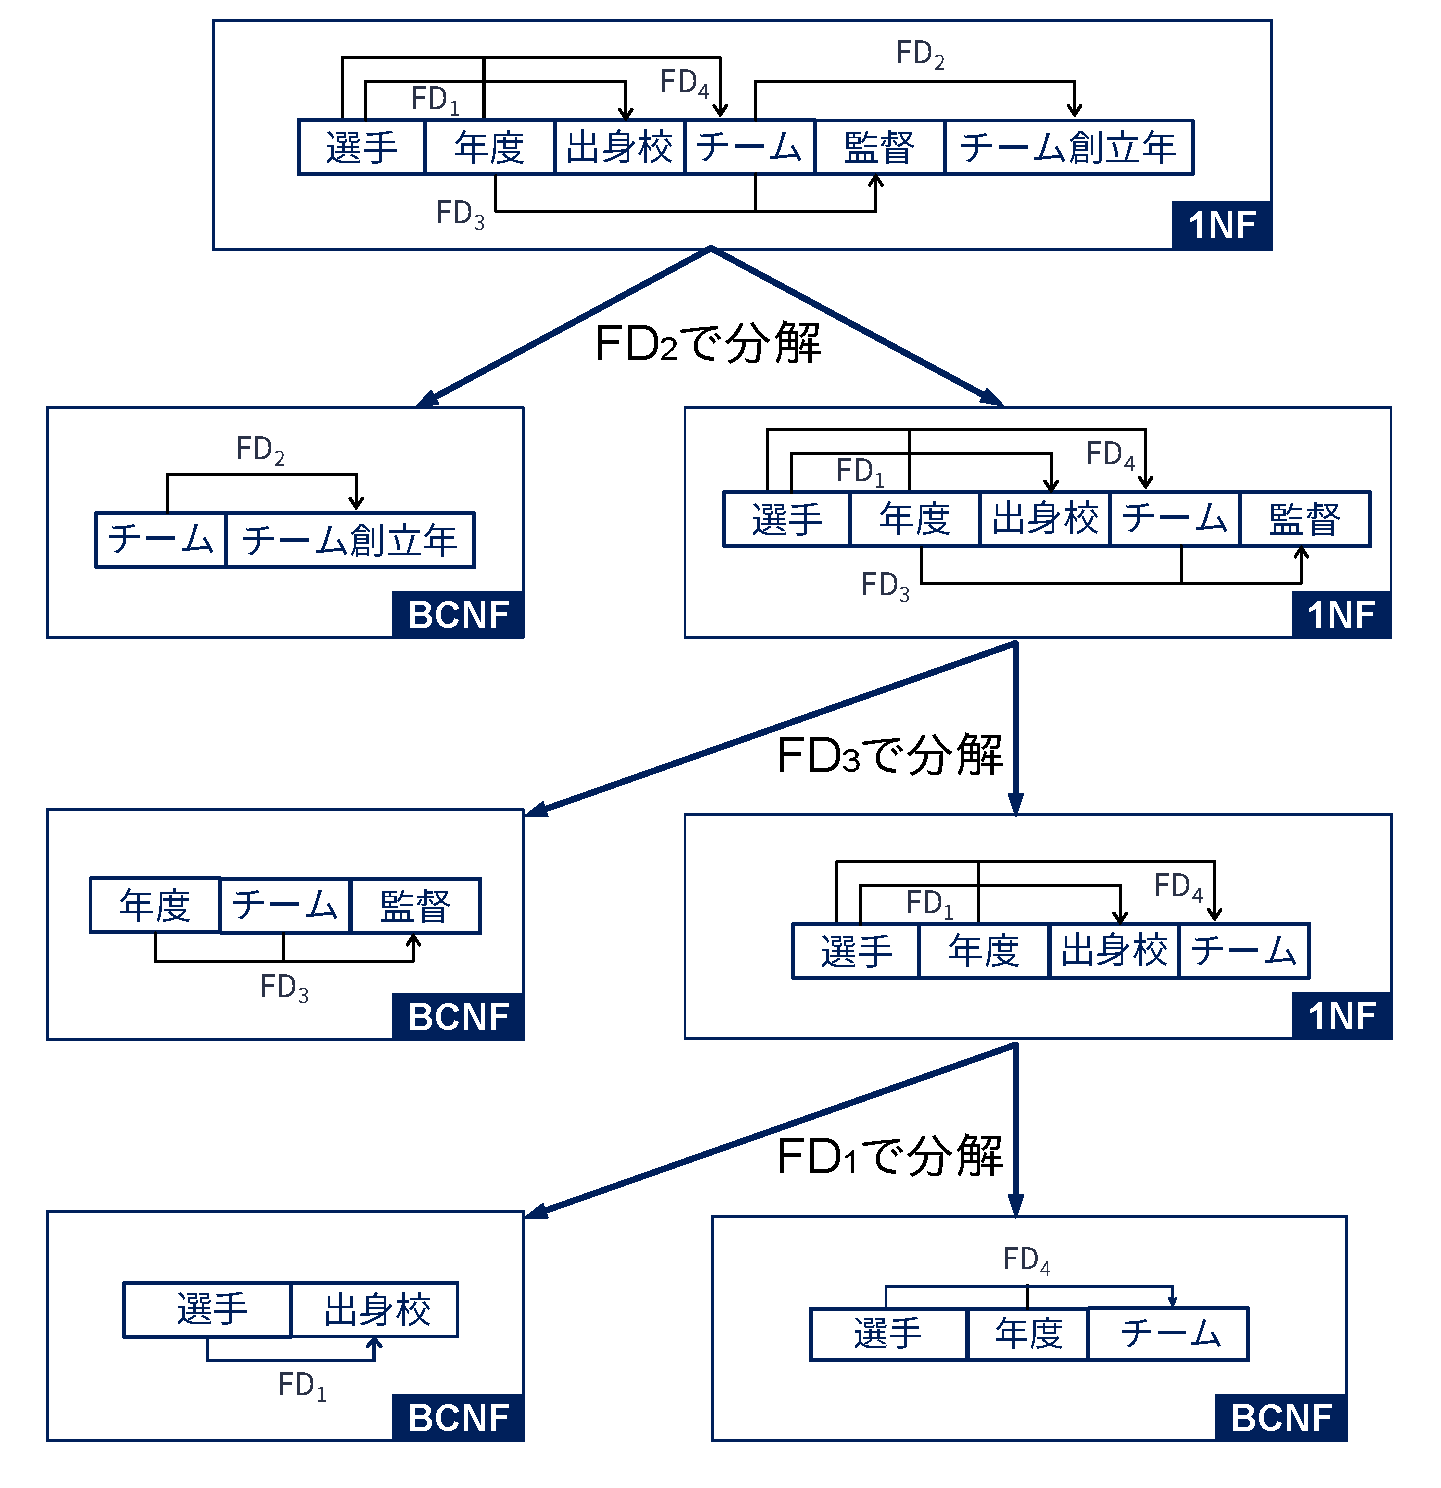
\includegraphics[width=0.90\textwidth]{figure/quiz-answer/ch7-q4.pdf}
    \caption{7章Q4の分解過程}
    \label{fig:ch7-q4}
\end{figure}

最終的に得られる4つのBCNFスキーマ：
\begin{align}
    &R_1(\underline{\text{選手}},\; \text{出身校}) \\
    &R_2(\underline{\text{チーム}},\; \text{チーム創立年}) \\
    &R_3(\underline{\text{チーム, 年度}},\; \text{監督}) \\
    &R_4(\underline{\text{選手, 年度}},\; \text{チーム})
\end{align}


% ==============================================================
\subsection*{第8章 SQL - その2}
% ==============================================================

以下のSQL文は\graybox{SSDSE.db}内のテーブル\graybox{population}，\graybox{activity}，\graybox{university\_student\_population\_top10}を対象とする．

\subsubsection*{Q1. 集合演算（1/2）}
「大学学生数 $\geq$ 7万」かつ「小学校児童数 $\geq$ 30万」の条件を\graybox{AND}で組み合わせ，\graybox{DISTINCT}で都道府県名の重複を除く．
\begin{minted}[gobble=0,
    bgcolor=background,
    fontsize=\small,
    linenos=false,
    xleftmargin=0em]{sql}
SELECT DISTINCT 都道府県
FROM population
WHERE 大学学生数 >= 70000
  AND 小学校児童数 >= 300000;
\end{minted}

\subsubsection*{Q2. 集合演算（2/2）}
Q1の2条件をそれぞれ別のクエリで表し，\graybox{INTERSECT}でその共通部分（積集合）を求める．
\begin{minted}[gobble=0,
    bgcolor=background,
    fontsize=\small,
    linenos=false,
    xleftmargin=0em]{sql}
SELECT DISTINCT 都道府県
FROM population
WHERE 大学学生数 >= 70000
INTERSECT
SELECT DISTINCT 都道府県
FROM population
WHERE 小学校児童数 >= 300000;
\end{minted}

\subsubsection*{Q3. 直積}
\graybox{CROSS JOIN}または\graybox{FROM}句に2テーブルをカンマ区切りで列挙することで直積を求める．
\begin{minted}[gobble=0,
    bgcolor=background,
    fontsize=\small,
    linenos=false,
    xleftmargin=0em]{sql}
SELECT *
FROM population
CROSS JOIN activity;
\end{minted}

\subsubsection*{Q4. 内部結合}
両テーブルに共通する列「地域コード」と「都道府県」の重複を避けるため，テーブルエイリアスを用いて必要な列を明示的に列挙する．
\begin{minted}[gobble=0,
    bgcolor=background,
    fontsize=\small,
    linenos=false,
    xleftmargin=0em]{sql}
SELECT p.地域コード, p.都道府県,
       p.調査年度, p.総人口,
       p.小学校児童数, p.中学校生徒数,
       p.高等学校生徒数, p.大学学生数,
       a.学習・自己啓発・訓練, a.スポーツ,
       a.趣味・娯楽, a.ボランティア, a.旅行・行楽
FROM population AS p
JOIN activity AS a ON p.地域コード = a.地域コード;
\end{minted}

\subsubsection*{Q5. 直積再び}
\graybox{JOIN}を用いず，\graybox{FROM}句に2テーブルをカンマ区切りで列挙して直積を作り，\graybox{WHERE}句で等結合の条件を指定する（Q4と同じ結果が得られる）．
\begin{minted}[gobble=0,
    bgcolor=background,
    fontsize=\small,
    linenos=false,
    xleftmargin=0em]{sql}
SELECT p.地域コード, p.都道府県,
       p.調査年度, p.総人口,
       p.小学校児童数, p.中学校生徒数,
       p.高等学校生徒数, p.大学学生数,
       a.学習・自己啓発・訓練, a.スポーツ,
       a.趣味・娯楽, a.ボランティア, a.旅行・行楽
FROM population AS p, activity AS a
WHERE p.地域コード = a.地域コード;
\end{minted}

\subsubsection*{Q6. 外部結合}
\graybox{university\_student\_population\_top10}を左テーブルとして\graybox{LEFT OUTER JOIN}する．テーブル\graybox{activity}に対応する地域コードがなければ，活動に関する列は\graybox{NULL}となる．
\begin{minted}[gobble=0,
    bgcolor=background,
    fontsize=\small,
    linenos=false,
    xleftmargin=0em]{sql}
SELECT u.地域コード, u.都道府県, u.総人口,
       a.学習・自己啓発・訓練, a.スポーツ,
       a.趣味・娯楽, a.ボランティア, a.旅行・行楽
FROM university_student_population_top10 AS u
LEFT OUTER JOIN activity AS a
  ON u.地域コード = a.地域コード;
\end{minted}

\subsubsection*{Q7. 副問い合わせ（1/2）}
\graybox{WITH}句（または副問い合わせ）で調査年度2021の小学校児童数上位20件を先に絞り込み，その結果とテーブル\graybox{activity}を結合する．
\begin{minted}[gobble=0,
    bgcolor=background,
    fontsize=\small,
    linenos=false,
    xleftmargin=0em]{sql}
WITH top20 AS (
    SELECT *
    FROM population
    WHERE 調査年度 = 2021
    ORDER BY 小学校児童数 DESC
    LIMIT 20
)
SELECT top20.*, a.学習・自己啓発・訓練, a.スポーツ,
       a.趣味・娯楽, a.ボランティア, a.旅行・行楽
FROM top20
JOIN activity AS a ON top20.地域コード = a.地域コード;
\end{minted}

\subsubsection*{Q8. 副問い合わせ（2/2）}
まず\graybox{WITH}句でボランティア活動率が上位10件以内の都道府県を求め，その都道府県について\graybox{population}テーブルから調査期間（2020年・2021年）の平均総人口を算出する．
\begin{minted}[gobble=0,
    bgcolor=background,
    fontsize=\small,
    linenos=false,
    xleftmargin=0em]{sql}
WITH top_volunteer AS (
    SELECT 地域コード
    FROM activity
    ORDER BY ボランティア DESC
    LIMIT 10
)
SELECT p.都道府県, AVG(p.総人口) AS 平均総人口
FROM population AS p
JOIN top_volunteer AS tv ON p.地域コード = tv.地域コード
GROUP BY p.都道府県;
\end{minted}
